\documentclass{article}

\thispagestyle{empty}
\usepackage[scale=.95]{geometry}

\usepackage{amsmath}
\usepackage{fontspec}
\usepackage{unicode-math}
\setmainfont{TeX Gyre Bonum}
\setmathfont{TeX Gyre Bonum Math}

\usepackage{tcolorbox}
\usepackage{varwidth}

\usepackage{tikz}
\usetikzlibrary{
  matrix,
  matrix.skeleton,
  decorations.pathreplacing,
  calligraphy,
  positioning,
  arrows.meta,
  calc,
  fit,
  tikzmark
}

\usepackage{siunitx}
\usepackage{tikzpagenodes}
\usepackage{accents}
\newcommand*{\dt}[1]{%
  \accentset{\mbox{\huge\bfseries .}}{#1}}
\newcommand*{\ddt}[1]{%
  \accentset{\mbox{\large\bfseries .\hspace{-0.25ex}.}}{#1}}

\ExplSyntaxOn

\seq_new:N \l__dec_dots_seq
\tl_new:N \l__dec_dots_a_tl
\tl_new:N \l__dec_dots_z_tl
\cs_new_protected_nopar:Npn \dec_dots:n #1
{
  \int_compare:nTF
  {
    \tl_count:n {#1} = 1
  }
  {
    \dt{#1}
  }
  {
    \seq_set_split:Nnn \l__dec_dots_seq {} {#1}
    \seq_pop_left:NN \l__dec_dots_seq \l__dec_dots_a_tl
    \seq_pop_right:NN \l__dec_dots_seq \l__dec_dots_z_tl
    \dt{\tl_use:N \l__dec_dots_a_tl}
    \seq_use:Nn \l__dec_dots_seq {}
    \dt{\tl_use:N \l__dec_dots_z_tl}
  }
}

\cs_new_nopar:Npn \dec_gcd:Nnn #1#2#3
{
  \int_compare:nNnTF {#2} > {#3}
  {\__dec_gcd:Nnn #1 {#2} {#3}}
  {\__dec_gcd:Nnn #1 {#3} {#2}}
}

\cs_new_nopar:Npn \__dec_gcd:Nnn #1#2#3
{
  \int_compare:nNnTF {#3} = {0}
  {\int_set:Nn #1 {#2}} {
    \dec_gcd:Nxn #1 {\int_eval:n {#2-#3}}{#3}
  }
}

\cs_generate_variant:Nn \dec_gcd:Nnn {Nxn, NVV}

\int_new:N \l__dec_tmpa_int
\int_new:N \l__dec_tmpb_int
\int_new:N \l__dec_tmpc_int
\tl_new:N \l__dec_tmpa_tl
\tl_new:N \l__dec_tmpb_tl

\NewDocumentCommand\DecimalRow {m m m}
{
  \(x = #1.#2\dec_dots:n{#3}\) \&
  \(x = #1.#2
  \int_compare:nTF {\tl_count:n {#3} = 1}
  {#3#3#3}
  {#3#3}
  \dots\) \&
  \(\int_compare:nF {\tl_count:n {#2} = 0}
  {1\prg_replicate:nn {\tl_count:n {#2}} {0}}
  x = #1#2.
  \int_compare:nTF {\tl_count:n {#3} = 1}
  {#3#3#3}
  {#3#3}
  \dots
  \) \&
  \(\int_compare:nF {\tl_count:n {#2#3} = 0}
  {1\prg_replicate:nn {\tl_count:n {#2#3}} {0}}
  x = \int_compare:nNnF{#1}={0}{#1}#2#3.
  \int_compare:nTF {\tl_count:n {#3} = 1}
  {#3#3}
  {#3}
  \dots\) \&
  \(\prg_replicate:nn {\tl_count:n {#3}} {9}
  \prg_replicate:nn {\tl_count:n {#2}} {0}
  x = \int_eval:n {#1#2#3 - #1#2}\) \&
  \(x = \frac{\int_eval:n {#1#2#3 - #1#2}}{
    \prg_replicate:nn {\tl_count:n {#3}} {9}
    \prg_replicate:nn {\tl_count:n {#2}} {0}
  }\) \&
  \tl_set:Nx \l__dec_tmpa_tl {\int_eval:n {(#2#3 - 0#2)}}
  \tl_set:Nx \l__dec_tmpb_tl {\prg_replicate:nn {\tl_count:n {#3}} {9}\prg_replicate:nn {\tl_count:n {#2}} {0}}
  \int_set:Nn \l__dec_tmpa_int {\tl_use:N \l__dec_tmpa_tl}
  \int_set:Nn \l__dec_tmpb_int {\tl_use:N \l__dec_tmpb_tl}
  \dec_gcd:NVV \l__dec_tmpc_int \l__dec_tmpa_int \l__dec_tmpb_int
  \(x = \int_compare:nNnF{#1}={0}{#1}\frac{
    \int_eval:n {\l__dec_tmpa_int / \l__dec_tmpc_int}
  }{
    \int_eval:n {\l__dec_tmpb_int / \l__dec_tmpc_int}
  }
  \)
}

\ExplSyntaxOff

\tikzset{
  >=Latex,
  show cell/.style 2 args={
    row #1 column #2/.style={
      every node/.append style={text opacity=1}
    },
  },
  current row/.initial=1,
  step current row/.style={
    current row/.expanded={\the\numexpr\pgfkeysvalueof{/tikz/current row}+1\relax}
  },
  show cell on current row/.style={
    show cell={\pgfkeysvalueof{/tikz/current row}}{#1}
  },
  show cells/.style 2 args={
    current row=#1,
    show cell on current row/.list={#2}
  },
  show cells on next row/.style={
    step current row,
    show cell on current row/.list={#1}
  }
}

\begin{document}

\begin{tcolorbox}[title=Template]
Let
%
\begin{align*}
x &= 8.2\dt{5}\dt{4} \tikzmark{col1} \\
&= 8.25454\dots \tikzmark{col2}
\end{align*}
%
Then
%
\begin{align*}
10 x &= 82.5454\dots \tikzmark{col3} \\
\num{1000} x &= 8254.5454\dots \tikzmark{col4}
\end{align*}
%
So
%
\begin{align*}
\num{990} x &= 8172 \tikzmark{col5} \\
x &= \frac{8172}{990} \tikzmark{col6} \\
&= 8 \frac{14}{55} \tikzmark{col7}
\end{align*}

\begin{tikzpicture}[remember picture, overlay]
\foreach \k in {1,...,7}
{
  \draw[->] let \p1=(current page text area.east), \p2=(pic cs:col\k) in (\x1,\y2)
  node[
    anchor=base east,
    name={lbl\k},
    node contents={\emph{Column \(\k\)}}
  ]
  (lbl\k) -- (lbl\k -| \x2+2em,\y2)
  ;
}
\end{tikzpicture}

\end{tcolorbox}

\begin{center}
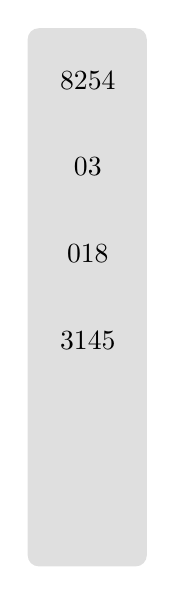
\begin{tikzpicture}
\matrix[
  matrix of nodes,
  ampersand replacement=\&,
  nodes={inner xsep=2mm, minimum width=.8cm,text opacity=0,minimum height=1.1cm},
  style odd tiling columns={fill=gray!25,rounded corners},
  %
  row 1/.style={every node/.append style={text opacity=1}},
  %
  current row=1,
  show cells on next row={1},
  show cells on next row={1},
  show cells on next row={1},
  show cells on next row={4},
  show cells on next row={5},
]
(m)
{
  \DecimalRow{8}{2}{54} \\
  \DecimalRow{0}{}{3} \\
  \DecimalRow{0}{}{18} \\
  \DecimalRow{3}{1}{45} \\
  \DecimalRow{7}{3}{18} \\
  \DecimalRow{11}{}{132} \\
};

\end{tikzpicture}
\end{center}



\end{document}
